%%%%%%%%%%%%%%%%%%%%%%%%%%%%%%%%%%%%%%%%%%%%%%%%%%%%%%%%%%%%%%%%%%%%%%%%%%%%%%%%
\section{Supplementary materials}
%%%%%%%%%%%%%%%%%%%%%%%%%%%%%%%%%%%%%%%%%%%%%%%%%%%%%%%%%%%%%%%%%%%%%%%%%%%%%%%%

\begin{figure}[!htbp]
  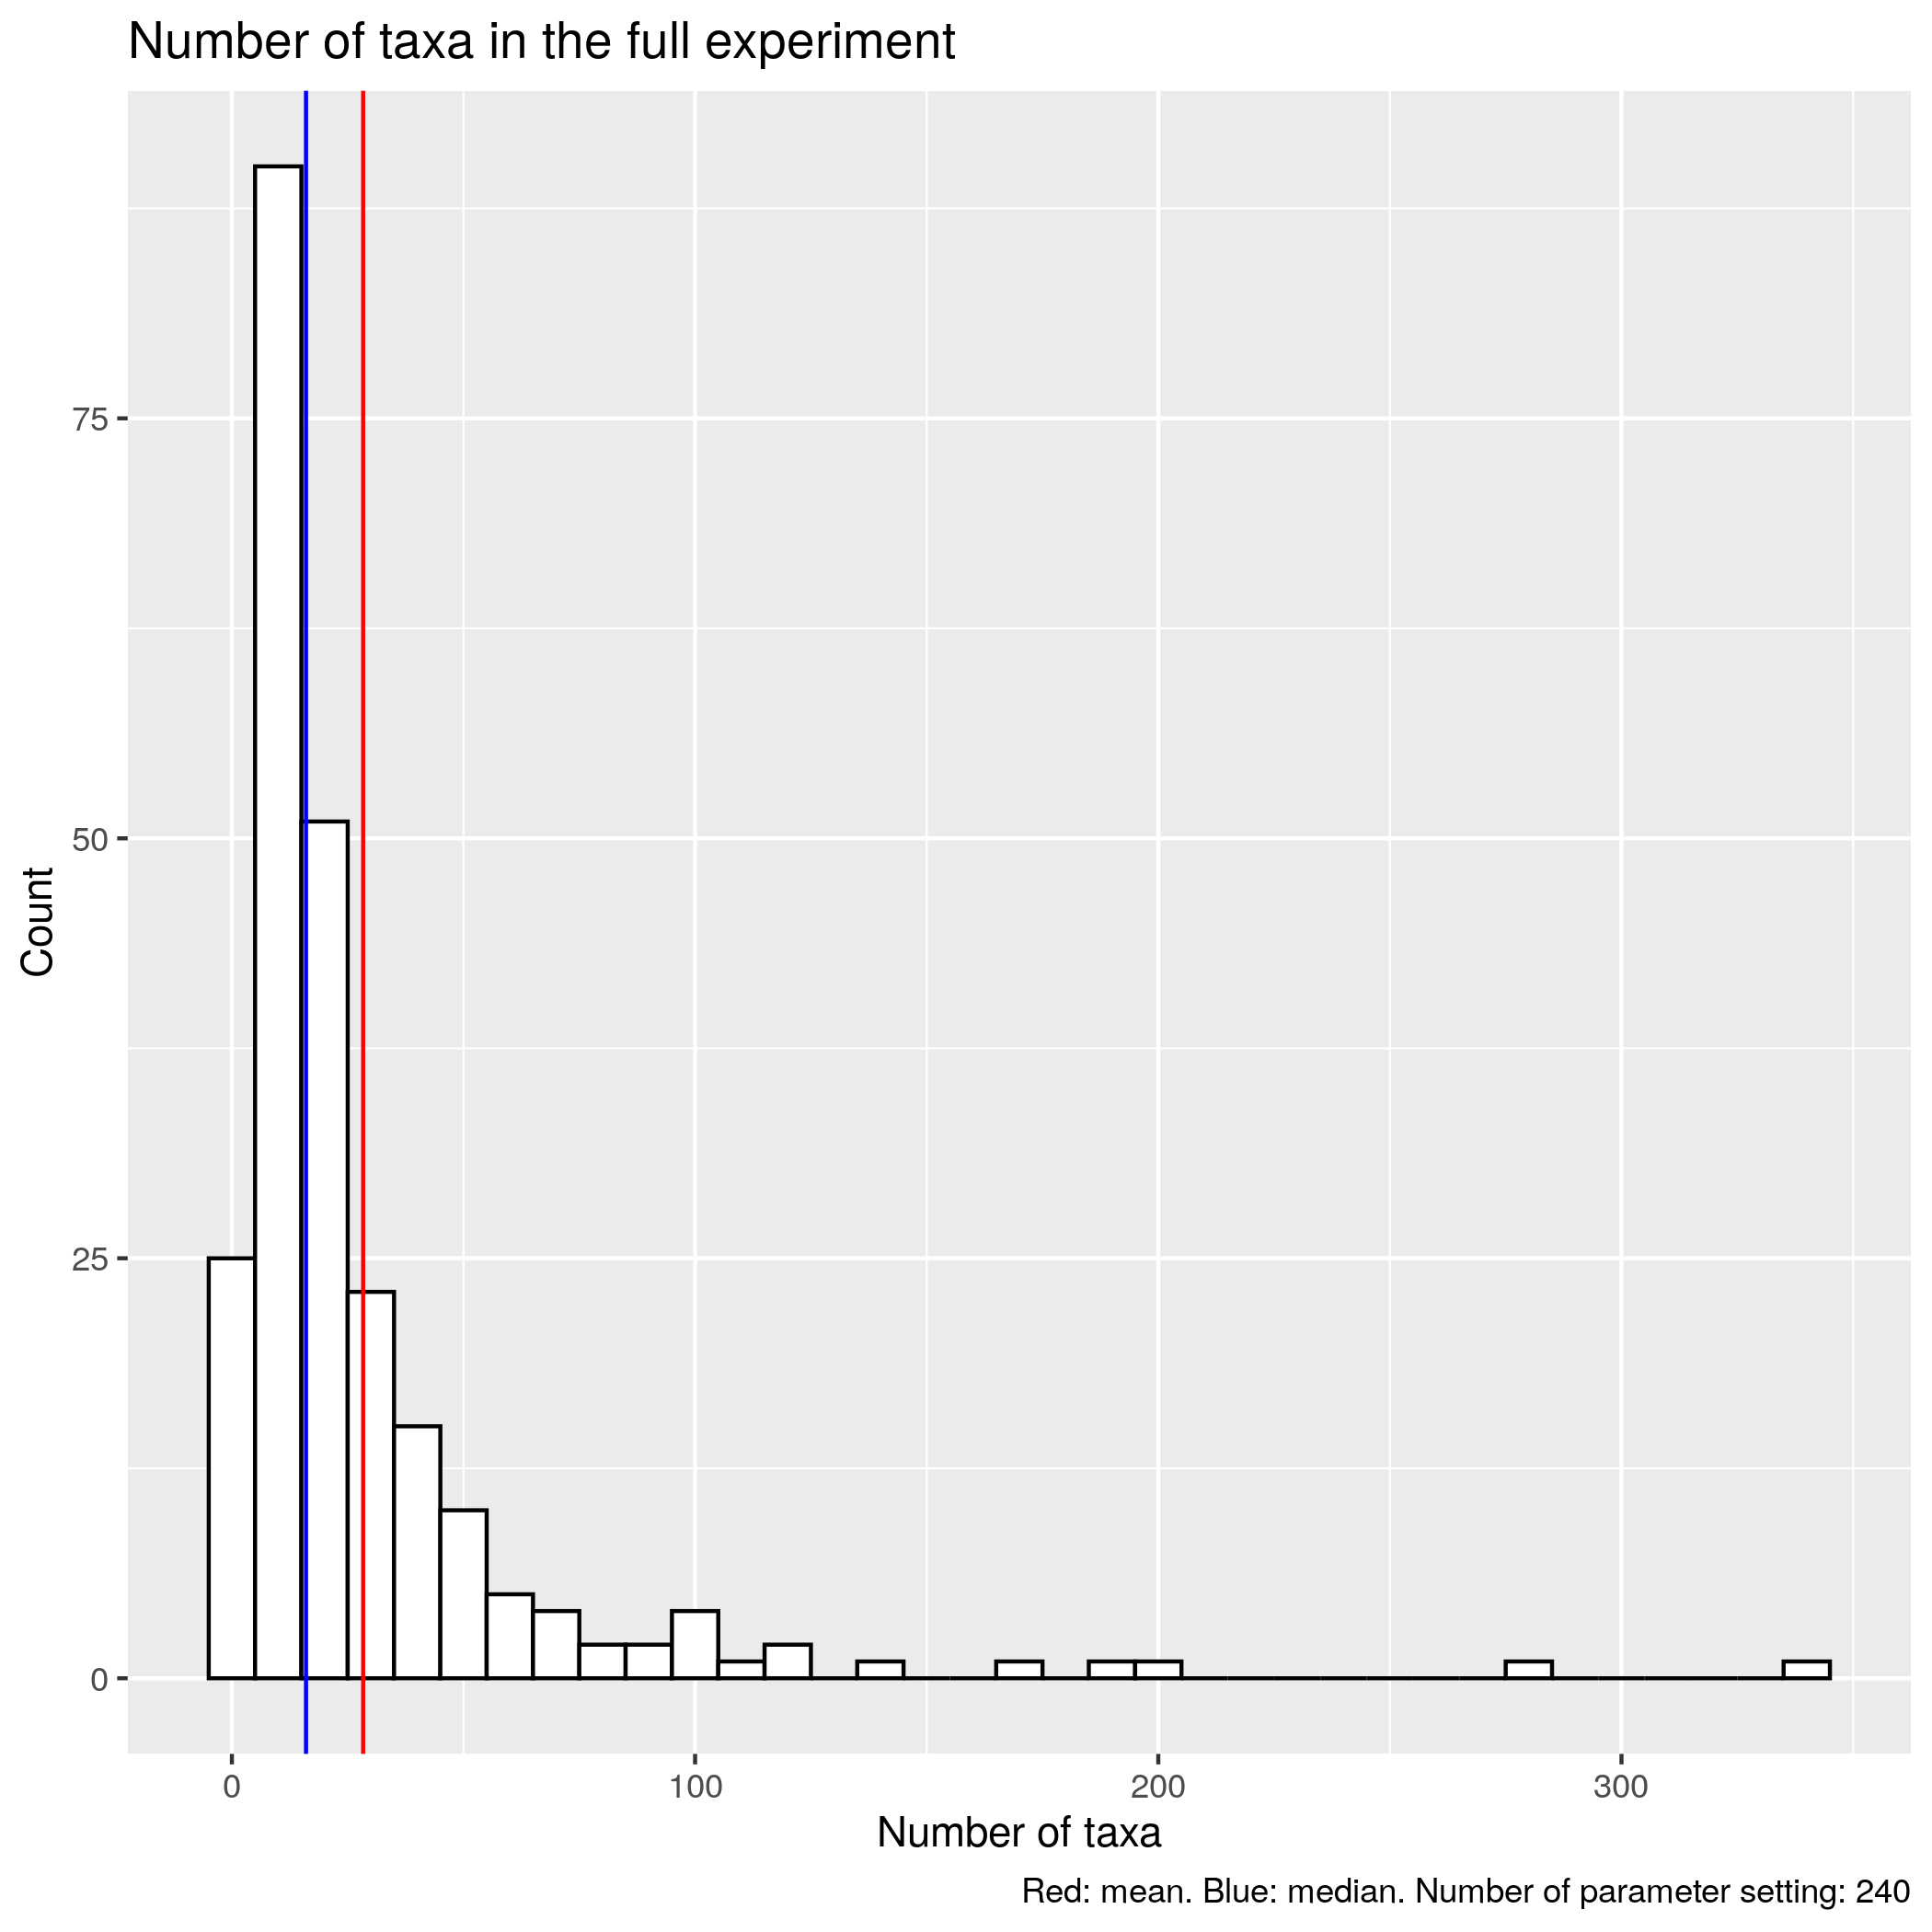
\includegraphics[width=\textwidth]{20190905_fig_n_taxa.png}
  \label{fig:n_taxa}
\end{figure}

\begin{figure}[!htbp]
  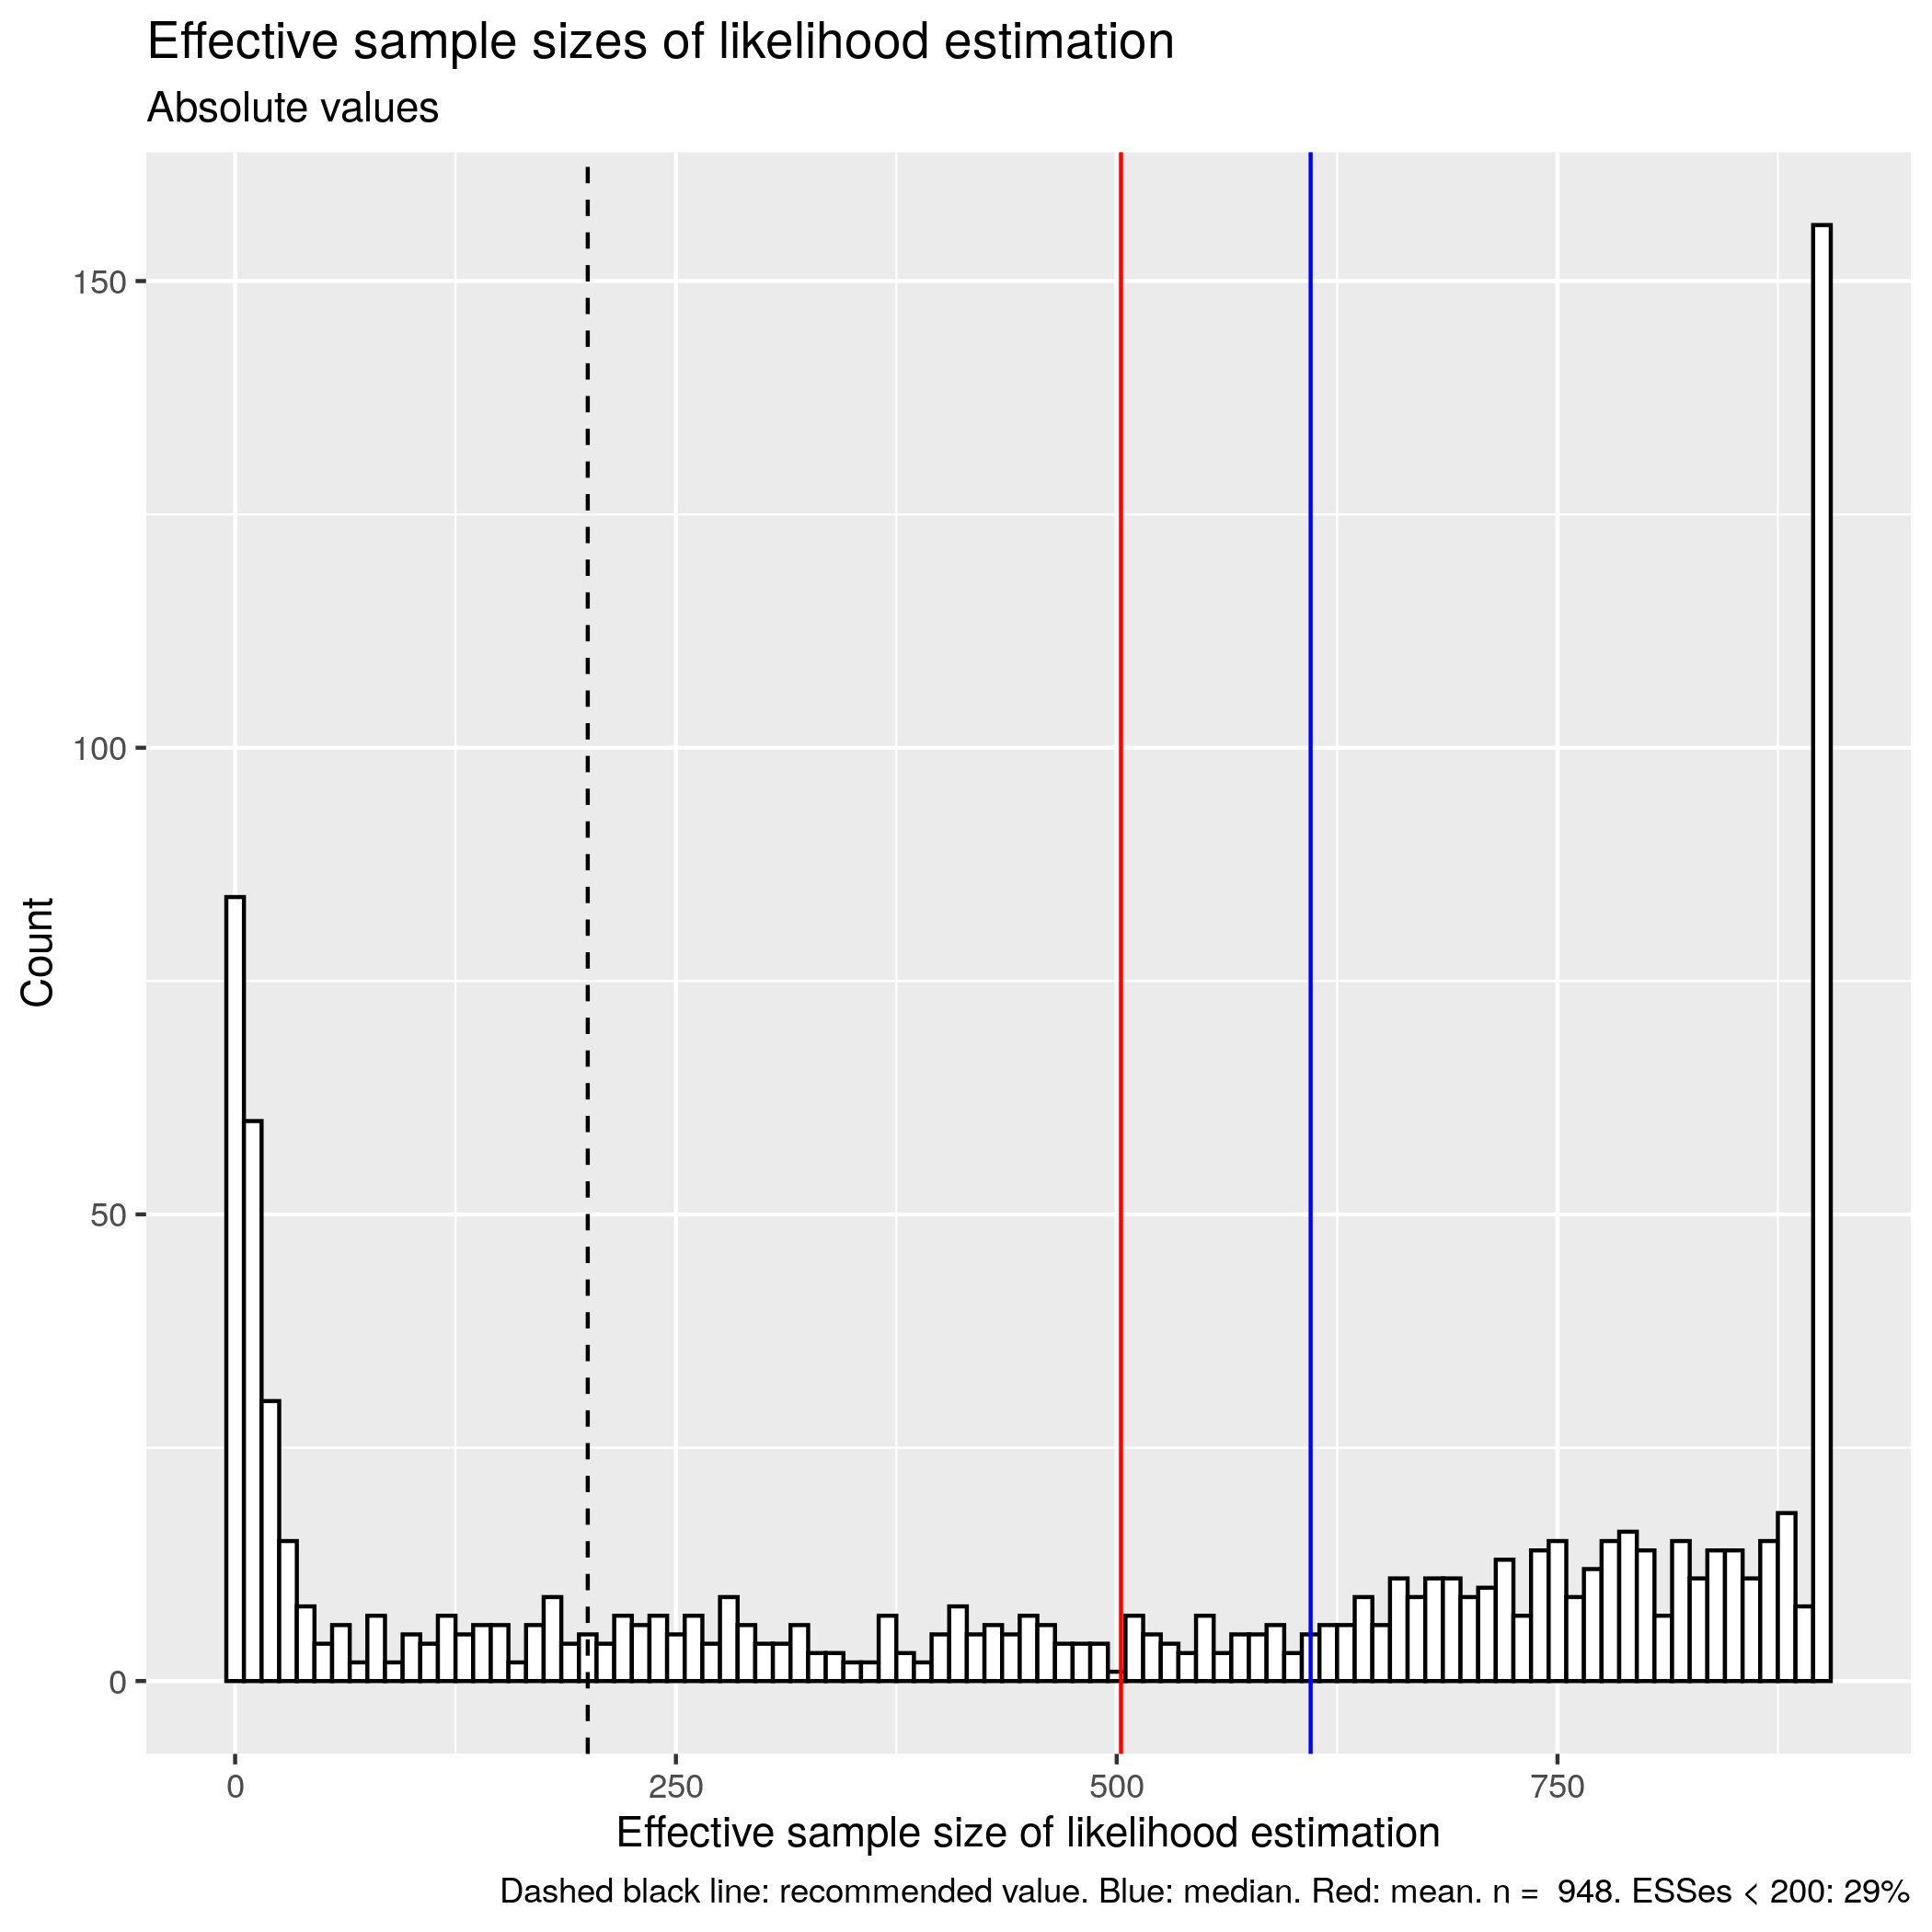
\includegraphics[width=\textwidth]{20190905_fig_esses.png}
  \label{fig:esses}
\end{figure}

\begin{figure}[!htbp]
  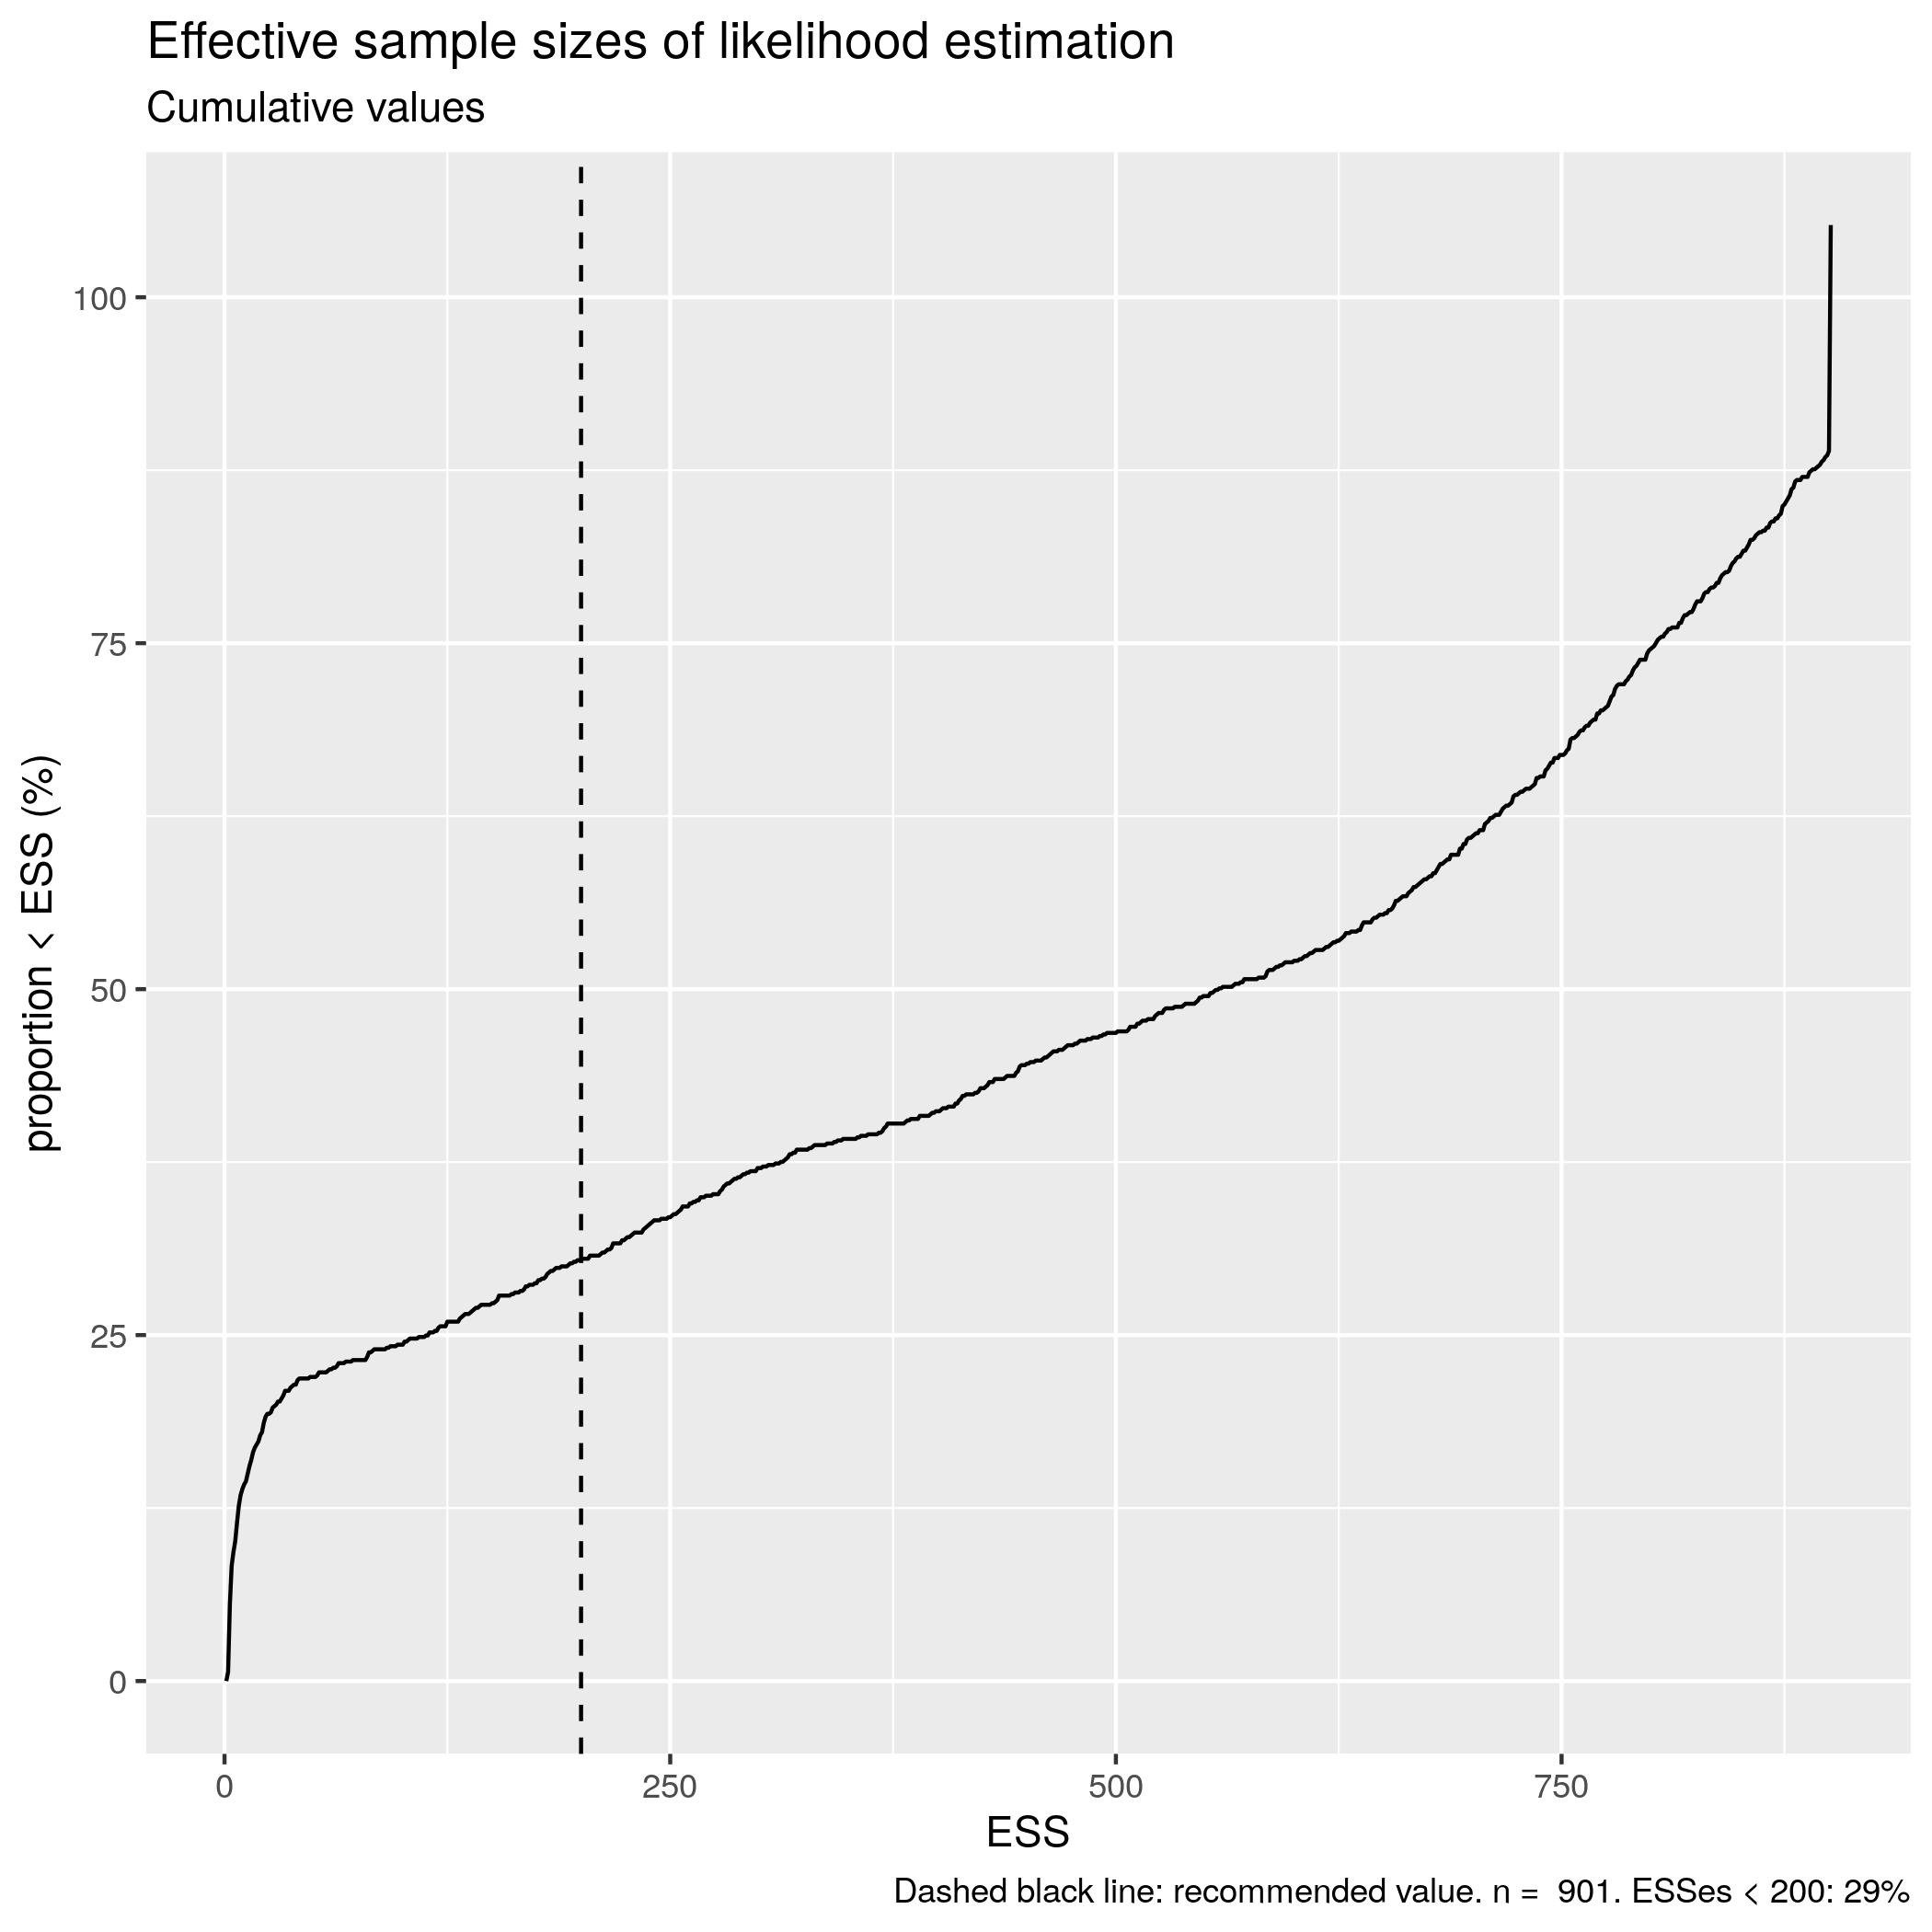
\includegraphics[width=\textwidth]{20190905_fig_esses_cumulative.png}
  \label{fig:esses_cumulative}
  \caption{\richel{n = 901 is something sloppy: the maximum ESS is 901. Next
    to that, the number of ESSes is approx 946}}
\end{figure}

\begin{figure}[!htbp]
  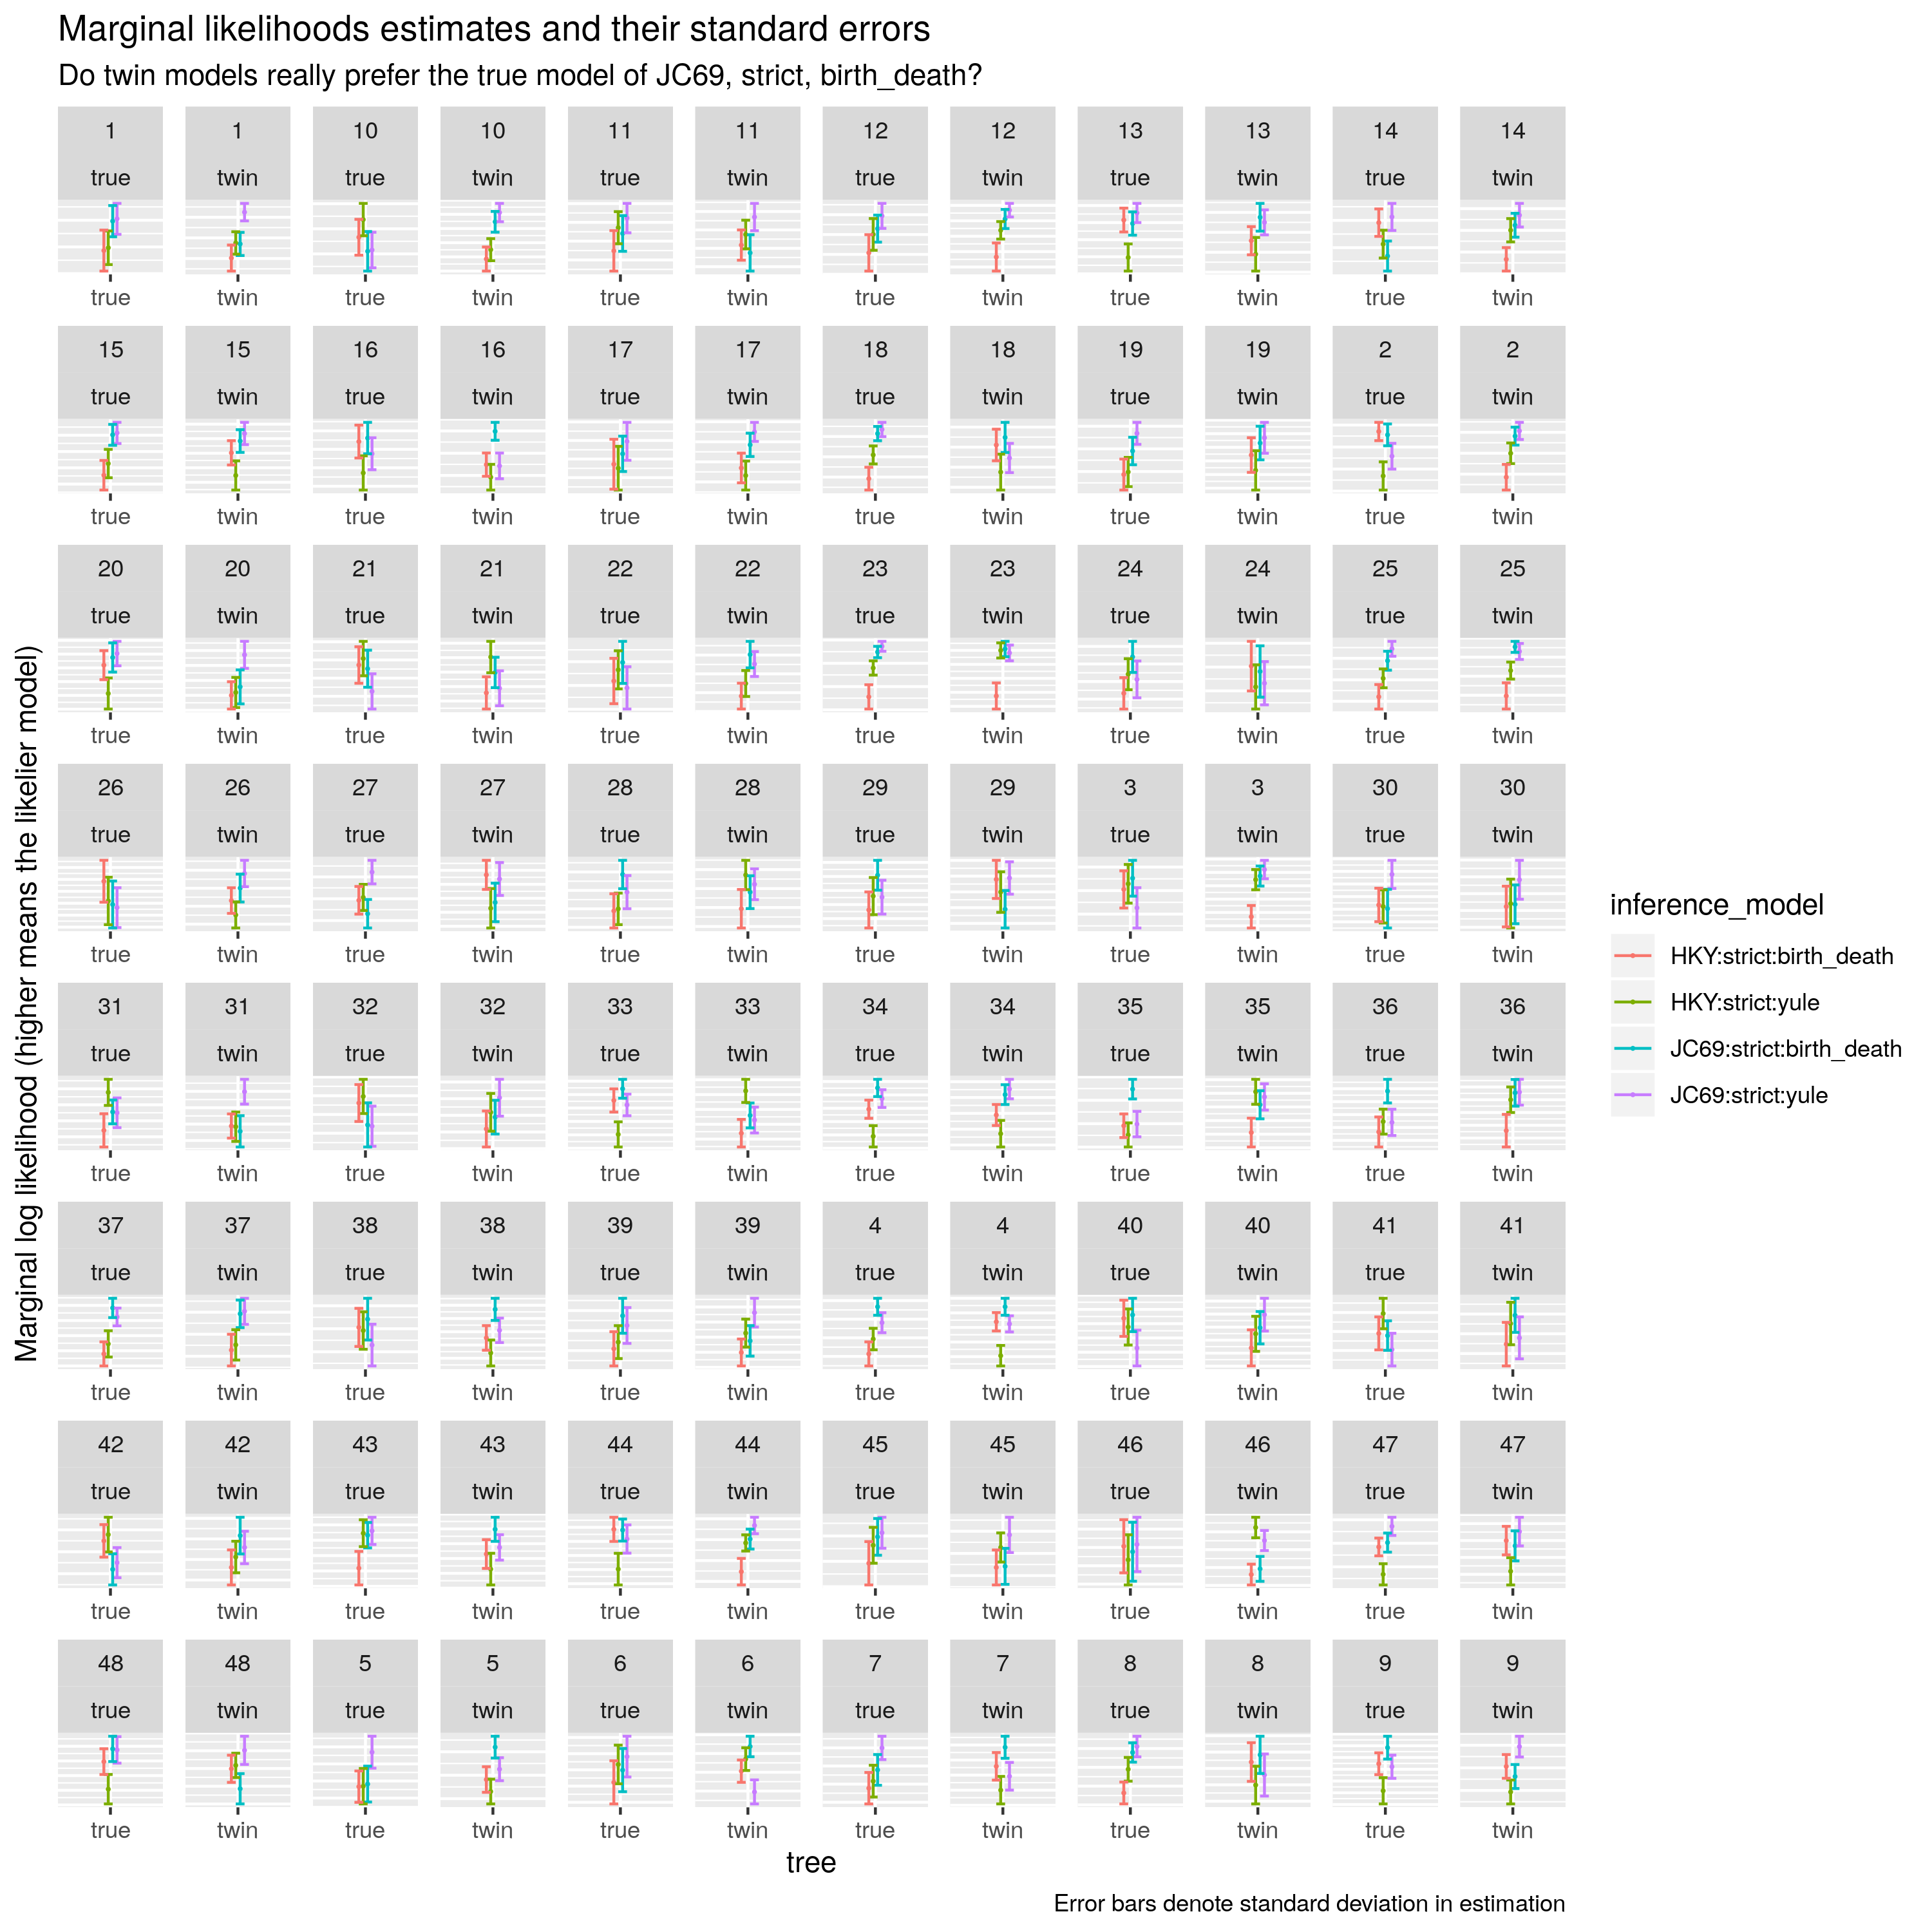
\includegraphics[width=\textwidth]{20190904_fig_marg_liks.png}
  \label{fig:marg_liks}
  \caption{The log marginal likelihood estimations of the models and their
    standard deviation (on the y axis), separated for the true and twin tree. 
    The number above each plot shows the RNG seed. Because the actual value
    of the marginal likelihood is uninformative, the actual log marginal 
    likelihood values are omitted for readability.
    This figure shows the first two replicates per
    unique parameter setting.\richel{I think one replicate would be even
    better}
  }
\end{figure}




